\documentclass[11pt]{article}
%\markright{Official Use Only}
\usepackage{fancyhdr}
\usepackage{graphicx}
\usepackage{listings}
\usepackage{color}
\usepackage{enumitem}
\usepackage{hyperref}
\usepackage{verbatim}

\textwidth 7.0in
\textheight 9in
%\itemsep 0pt
%\parsep 3pt
%\parindent 5pt
\parskip 3pt
\hoffset -1.in
\voffset -0.5in

\pagestyle{fancy}
\fancyhf{}
\lhead{Systematic Error Study}
\rhead{July 2017}

%\usepackage{pdfsync}
\begin{document}
% Figure commands (not needed here)
\renewcommand{\textfraction}{0.1}
\renewcommand{\topfraction}{0.9}
\renewcommand{\bottomfraction}{0.9}
\renewcommand{\floatpagefraction}{0.1}

\begin{center}
{\Large \bf Systematic Error Study for ALICE charged-jet $v_2$ Measurement}\\
\bigskip
LLNL-TR-xxxxxx
\footnote{This work was performed under the auspices of the U.S. Department of Energy by Lawrence Livermore National Laboratory under Contract DE-AC52-07NA27344.}
\\
\bigskip
Matthias Heinz and Ron Soltz
\end{center}

\begin{abstract}
We study the treatment of systematic errors in the determination of $v_2$ for charged jets in $\sqrt{s_{NN}}=2.76$~TeV Pb-Pb collisions by the ALICE Collaboration~\cite{Adam:2016ix}. Working with the reported values and errors for the 0-5\% centrality data we evaluate the $\chi^2$ according to the formulas given for the statistical and systematic errors, where the latter are separated into correlated and shape contributions. We reproduce both the $\chi^2$ and $p$-values relative to a null (zero) result. We then re-cast the systematic errors into an equivalent co-variance matrix and obtain identical results, demonstrating that the two methods are equivalent. 
\end{abstract}

\section{Motivation}

This work is motivated by the need to select a data format that can accommodate a full range of systematic errors. To date, most high energy physics experiments publish results with estimates for both statistical and systematic errors of each bin, under the assumption that these errors are fully correlated across all bins. Some experiments are beginning to publish systematic errors as co-variance matrices, which are more general. In theory the former can be recast into the latter, more general format. Using the recently published charged-jet $v_2$ measurements from ALICE we show that evaluation $\chi^2$ using both methods yields consistent results.

\section{$\chi^2$ Minimization Method}

    \begin{figure}[h]
\begin{center}
        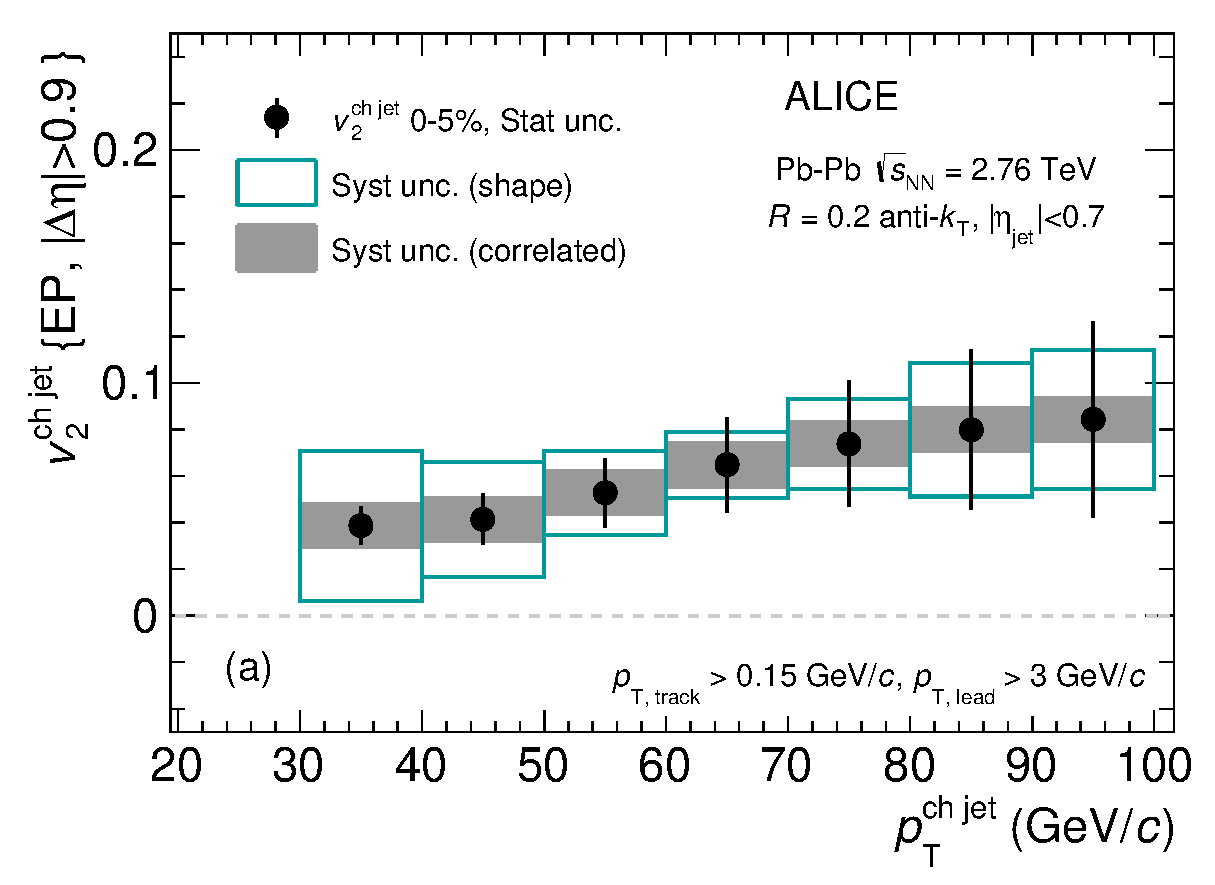
\includegraphics[width=.5\textwidth]{figures/data}
        \caption{Second-order harmonic coefficient $v_2^{ch\ jet}$ as a function of $p_T$) for 0--5\% collision centrality, reproduced from Fig.~4a of~\cite{Adam:2016ix}.  The error bars on the points represent statistical uncertainties, the open and shaded boxes indicate the shape and correlated uncertainties as explained in Sec.~2.5 of~\cite{Adam:2016ix}.}
        \label{fig:data}
\end{center}
    \end{figure}

The significance test calculation done by the ALICE collaboration used the following equation:
\begin{equation}\label{eq:chisq_org}
    \tilde{\chi}^2 (\epsilon_{corr}, \epsilon_{shape}) = \left[ \left( \sum_{i=1}^{n} \frac{(v_{2, i} + \epsilon_{corr} \sigma_{corr, i} + \epsilon_{shape} - \mu_i)^2}{\sigma^2_i} \right)+ \epsilon_{corr}^2 +  \frac{1}{n}\sum_{i=1}^{n} \frac{\epsilon_{shape}^2}{\sigma^2_{shape, i}}   \right]
\end{equation}
$\mu_i$ is the hypothesis against which we are testing the data, which is 0 in our case. $\sigma_{corr, i}$ and $\sigma_{shape, i}$ are the correlated and shape uncertainties on the $i$-th bin, and $\sigma_i$ is the uncorrelated uncertainty on the $i$-th bin. $\epsilon_{corr}$ and $\epsilon_{shape}$ are free parameters with respect to which the $\tilde{\chi}^2$ is minimized. This minimization was done using the \texttt{iminuit} package in Python. Using the minimized $\tilde{\chi}^2$, the $p$-value was obtained by using the \texttt{chisqprob} method with $n - 2$ degrees of freedom from the Python scipy statistics library. Using this approach, we were able to verify the results published by the ALICE collaboration.

\begin{table}[h]
\begin{center}
\begin{tabular}{ l r r }
  & \multicolumn{2}{c}{$p$-value} \\
$p_T$ range & ALICE & LLNL \\
\hline
30-100 GeV & 0.12 & 0.12 \\ 
30-60 GeV & 0.07 & 0.07 \\ 
60-100 GeV & 0.02 & 0.02 \\
% \hline
\end{tabular}
\caption{p-values as reported by ALICE in~\cite{Adam:2016ix} and re-calculated using~Eq.\ref{eq:chisq_org}.}
\end{center}
\end{table}

\section{Co-Variance Method}

It can be shown that (\ref{eq:chisq_org}) can be re-expessed in the form:
\begin{equation}\label{chisq_eff}
    \tilde{\chi}^2 (\epsilon_{corr}, \epsilon_{new}) = \left[ \left( \sum_{i=1}^{n} \frac{(v_{2, i} + \epsilon_{corr} \sigma_{corr, i} + \epsilon_{new} \sigma_{new} - \mu_i)^2}{\sigma^2_i} \right)+ \epsilon_{corr}^2 + \epsilon_{new}^2 \right]
\end{equation}
\begin{equation}\label{sigma_new}
    \sigma_{new} = \frac{1}{n}\sum_{i=1}^{n} \frac{1}{\sigma^2_{shape, i}}
\end{equation}
\begin{equation}\label{eps_new}
    \epsilon_{new} = \frac{\epsilon_{shape}}{\sigma_{new}}
\end{equation}
$\sigma_{new}$ is effectively a uniform, fully-correlated error, indepedent from $\sigma_{corr, i}$. With the $\chi^2$ expressed in this form, we map this to an equivalent covariance matrix formulation of the minimization, following the derivations given in~\cite{Demortier:1999aa,Gao:2014cp}, where this equivalence has been shown to be exact in cases where the minimization formulation is performed without constraints.  With the covariance matrix:
\begin{equation}\label{covariance_matrix}
    C_{ij} = \sigma_i^2 \delta_{ij} + \sigma_{corr, i} \sigma_{corr, j} + \sigma_{new} \sigma_{new}
\end{equation}
the minimized $\chi^2$ can be calculated by:
\begin{equation}\label{cov_mat_chi2_min}
    \chi_{min}^2 = \Delta^T C^{-1} \Delta
\end{equation}
where $\Delta$ is a length-$n$ vector with:
\begin{equation}\label{delta_def}
    \Delta_i = v_{2, i} - \mu_i
\end{equation}
Again, the $p$-value is computed from the $\chi_{min}^2$ using a $\chi^2$ distribution with $n - 2$ degrees of freedom. The results are identical to those obtained by the ALICE collaboration. It is important to note that the $p$-values calculated by both methods are equal to roughly machine precision, verifying the exact equivalence of the two methods.

\begin{table}[h]
\begin{center}
\begin{tabular}{ l r r }
  & \multicolumn{2}{c}{$p$-value} \\
$p_T$ range & \texttt{iminuit}-minimized & Covariance matrix \\
\hline
30-100 GeV & 0.1247858497 & 0.1247858497 \\ 
30-60 GeV & 0.0685915881 & 0.0685915881 \\ 
60-100 GeV & 0.0211009165 & 0.0211009165 \\
% \hline
\end{tabular}
\caption{p-values reported to machine level significance calculated using the minimization of Eq.~\ref{eq:chisq_org} and co-variance method of Eq.~\ref{cov_mat_chi2_min}.}
\end{center}
\end{table}

\bibliographystyle{plain}
\begin{thebibliography}{10}

\bibitem{Adam:2016ix} J. Adam {\it et al.} [ALICE Collaboration], Azimuthal anisotropy of charged jet production in $\sqrt{s_{NN}}$=2.76~TeV Pb-Pb collisions, {\it J. Phys. Lett. B}, 753, 511 (2016).

\bibitem{Demortier:1999aa} L. Demortier, Equivalence of the best-fit and covariance-matrix methods for comparing binned data with a model in the presence of correlated systematic uncertainties, CDF-MEMO-8661 (1999).

\bibitem{Gao:2014cp} J. Gao, {\it et al.}, CT10 next-to-next-to-leading order global analysis of QCD, {\it Phys. Rev. D} 89, 03309 (2014).

\end{thebibliography}

\end{document}